\section{Ma mission au sein du projet}
Ma mission au sein du projet fut donc de contribuer au développement d’une solution de collecte et stockage de données acquises sur les parcelles agricoles mises à la disposition des participants au challenge. 

Plus précisément, il s’agissait de concevoir, modéliser et implémenter une base de données qui servira à stocker les données collectées au moyen de capteurs implantés sur le site de Montoldre. Cette base de données pourra participer à un dispositif d’aide à la décision permettant aux participants du challenge de savoir à quel moment intervenir sur les parcelles et ainsi mettre en pratique leurs solutions de désherbage.  

L’un des points importants à cette mission était de rendre cette base de données assez générique pour pouvoir être alimenter par différents types de données provenant de différents types de capteurs. 

En parallèle à cette tâche, je devais également proposer une solution d’extraction, transformation de données capteurs météo déjà implantés. En effet, deux stations météo, ont été installé sur le site de Montoldre. Tout l’enjeu de cet exercice était de pouvoir automatiser, par le biais d’un programme, les tâches d’extraction et de transformation. Les données sont ainsi relevées sous leurs formats d’origine converties dans des formats standard avant d’être sauvegardées dans la base de données. 

Finalement, après avoir fait la base de données capteurs, et le programme extracto-chargeur, il fallait penser à la meilleure façon d’envoyer toutes ces données au LNE qui s’occupe de la mise à disposition de celles-ci aux participants du challenge. 

 
\subsection{Cahier des charges}
 \begin{itemize}
      \item Modéliser une base de données générique pouvant stocker n’importe quel type de données capteurs. 
     \item Extraire, transformer et stocker les données des capteurs météo déjà présentes sur le site de Montoldre.
     \item Automatiser la tâche précédente et la rendre disponible sur différents système d’exploitation. 
     \item Proposer une solution pour un envoi des données, régulier, au LNE.
     \item Produire une documentation assez précise pour des futurs utilisateurs. 
     \item Mettre à disposition un outil interne de visualisation des données. 
 \end{itemize}

\subsection{Analyse de l’existant} 
Étant arrivé presque en début de projet, il est évident que la plupart des tâches venaient juste d’être reparties. Cela m’a permis de m’approprier très rapidement le projet, ce qui m’a permis de le comprendre dans sa globalité et plus particulièrement mon sujet de stage.   

Quand j’ai commencé à travailler sur le projet OPEROSE, une étude sur le recensement des caractéristiques des capteurs avait déjà été menée en amont par  d’autres stagiaires et des permanents de l’IRSTEA. 

\subsection{Choix des outils et technologies}

Conscient que le projet OPEROSE devait réunir plusieurs acteurs de différents domaines répartis sur toute la durée du projet, le choix des technologies et outils utilisés se devait de suivre quelques critères pour permettre une bonne maintenabilité future. Voici quelques critères qui ont influencé nos choix : 
\begin{itemize}
 

  \item La technologie ou l’outil utilisé doit être choisi en équipe : en effet durant mon stage la technologie  utilisée n’était pas imposé. Je n’ai pas  voulu une technologie qui m’était plus familière ou dont j’avais plus l’habitude. Je me suis plus orienté vers les technologies déjà utilisées dans l'équipe Cela est valable par exemple pour le choix du langage de programmation utilisé. 

  \item Les logiciels utilisés, pour des raisons pratiques, se devaient d’être libre d’utilisation et gratuit. 

   \item Facile à utiliser : outils dont l’utilisation est intuitive pour réduire au maximum le temps d’apprentissage 
\end{itemize}
Ces critères m'ont permis de réduire mes choix technologiques et de ne pas me perdre dans une immense quantité d'outils disponibles. Cela m'a également permis de me dépasser en m'obligeant à m'adapter à de nouveaux outils qui ne m'étaient pas familiers.

L'image \ref{fig : Outils et Technologies utilisés}résume l’ensemble des outils et technologies utilisés 
\begin{figure}
\begin{center}
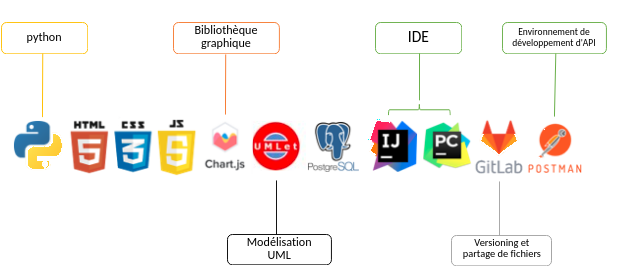
\includegraphics[width=400px]{images/logicielutilises.png}
\end{center}
\caption{Outils et Technologies utilisés}
\label{fig : Outils et Technologies utilisés}
\end{figure}
